\documentclass[10pt, preprint]{aastex}

\usepackage{natbib}
\bibliographystyle{apj}

\usepackage{minted}
\usepackage{float}
\usepackage{graphicx}
\usepackage{subfig}
\usepackage{amsmath}
\usepackage[toc,page]{appendix}
\usepackage[utf8]{inputenc}
\usepackage{hyperref}
\hypersetup{
    colorlinks=true,
    linkcolor=blue,
    filecolor=magenta,      
    urlcolor=blue,
    citecolor=blue,
}
\usepackage{booktabs}
\renewcommand{\arraystretch}{1}

\title{Assignment 2 - CTA200H}
\author{Rebecca Ceppas de Castro}

\begin{document}

\maketitle

\section*{Question 1}

For this question, two methods of numerical approximations for the derivative of $sin(x)$ at $x_0 = 0.1$ are compared to its analytical derivative. For reference, Equation \ref{method1} is called method 1 in the python script and it assumes $h$ is infinitesimally small. Equation \ref{method2} is referred to as method 2 and it more realistically assumes $h$ is a small but finite step size.

\begin{equation}\label{method1}
    d_xf|_{x_0} \approx \frac{f_{x_0 + h} - f_{x_0}}{h}
\end{equation}

\begin{equation}\label{method2}
    d_xf|_{x_0} \approx \frac{f_{x_0 + h} - f_{x_0 - h}}{2h}
\end{equation}

\begin{figure}[h]
    \centering
    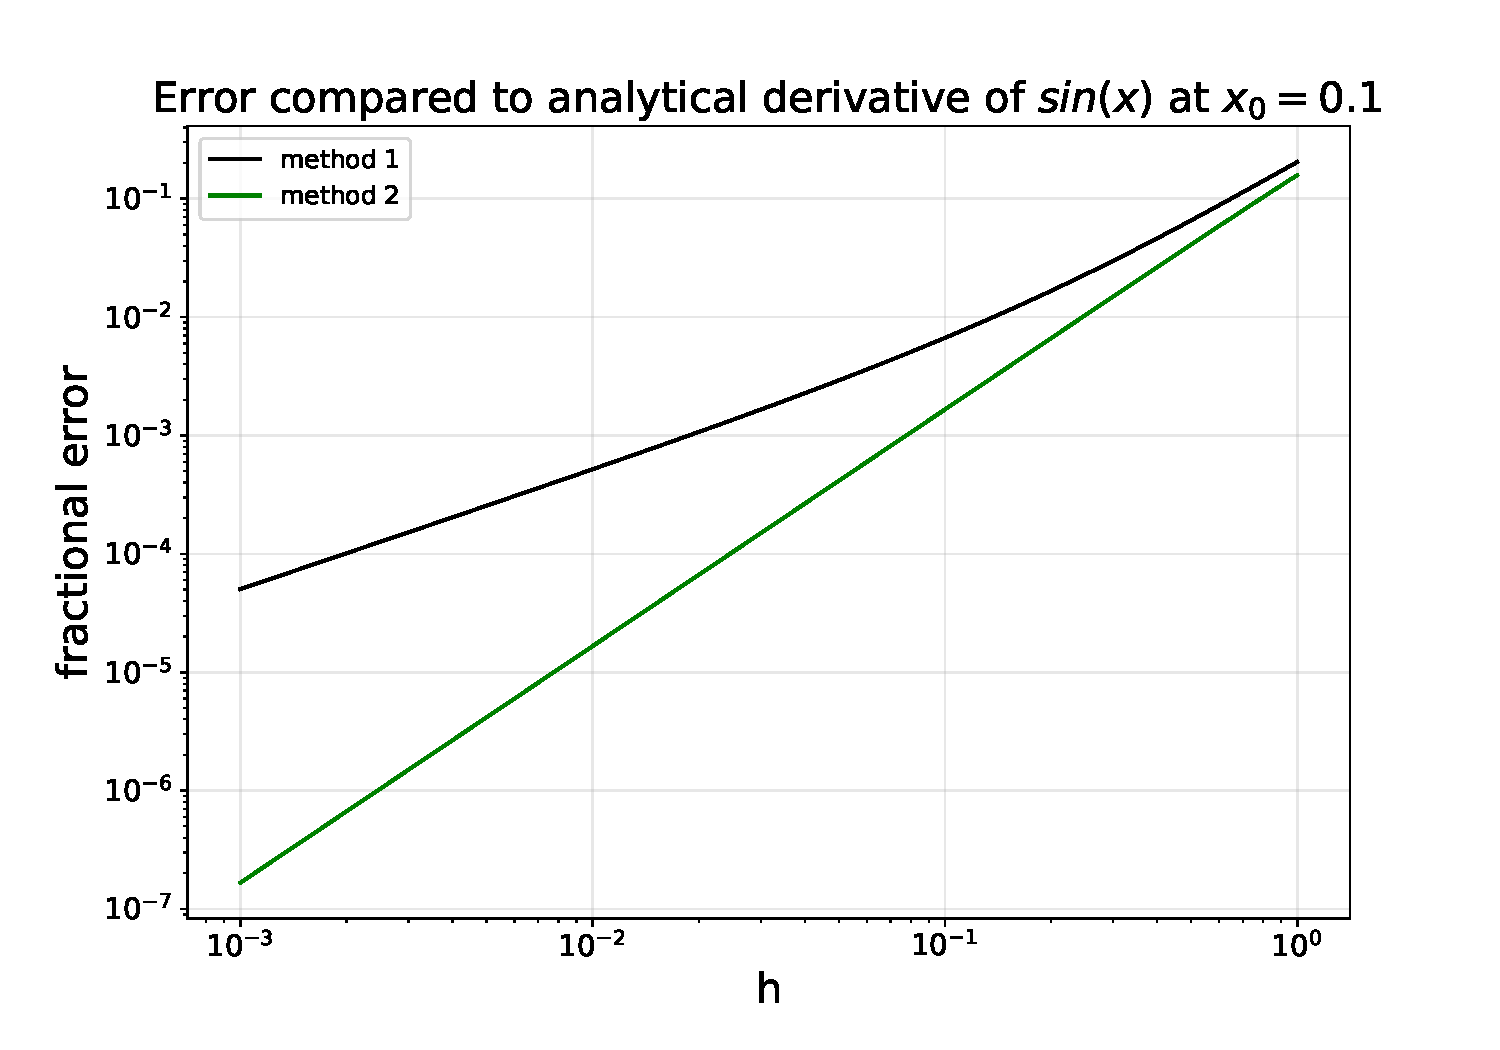
\includegraphics[width=0.7\textwidth]{derivatives.pdf}
    \caption{Comparison of the Fractional error resulting from using method 1 and method 2 with the analytical derivative of sin(x) at 0.1}
    \label{derivatives}
\end{figure}

Figure \ref{derivatives} shows that the fractional errors from both methods of numerical approximations are relatively small for small values of h and increase at different rates for higher values of h, as expected. The first to notice is that method 2 always has a smaller fractional error, which agrees with the fact that that method assumes h is finite and we, in fact, used finite values of h in the calculations. The slope shows that the error in the approximation when using method 2 is more susceptible to changes in h, while method 1 shows less of this variation. In other words, while both methods have high errors for large step sizes, using method 2 produces more accurate results at a faster rate than if you were using method 1 as you decrease the step size.

\section*{Question 2}

In this question, we plot the Mandelbrot set, obtained through the recurring relation $z_{i+1} = z_{i}^2 + c$, where $c$ is a complex number given by $c = x + iy$ for $-2 < x < 2$ and $-2 < y < 2$. For different complex numbers $c$, the set diverges after a certain number of iterations, while for others it is bounded. In my function \textit{get\_z}, I use try and except to keep track of the bounded sets, as well as the number of iterations ran through before the divergent sets diverged. For the bounded sets, I designated a value of 10000 iterations, as if I used the real value - infinite number of iterations before divergence - we would lose some details in Figure \ref{mandelbrot}.

\begin{figure}[h!]
    \centering
    \subfloat[Divergent and Bounded points c]{{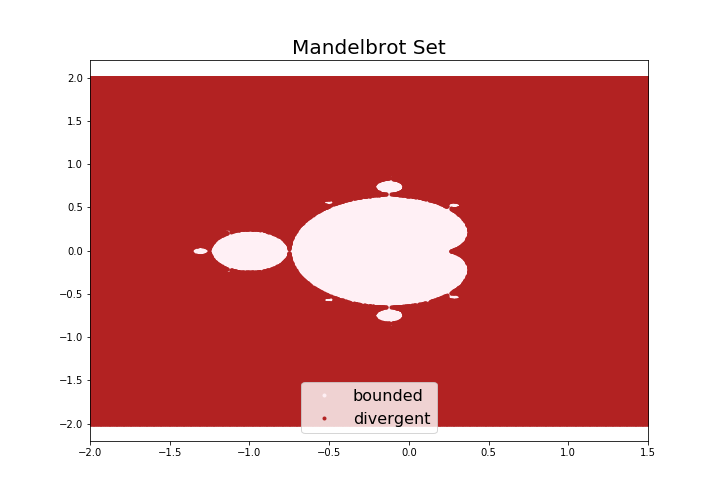
\includegraphics[width=0.5\textwidth]{duo.png}}}
    \hfill
    \subfloat[Mandelbrot Set with colour map based on number of iterations before divergence]{{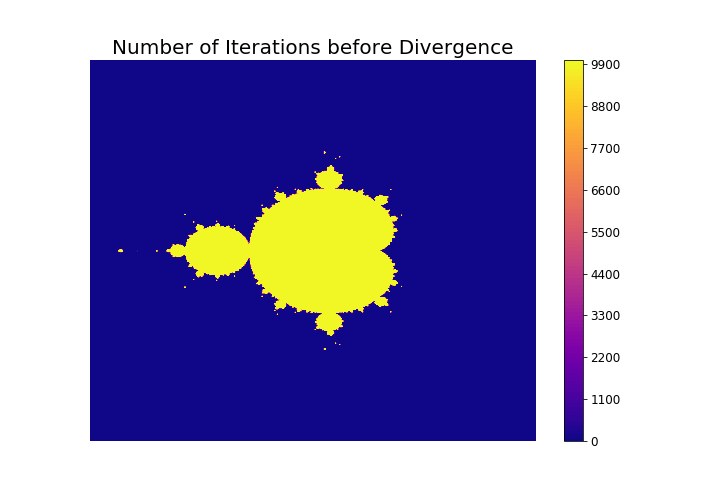
\includegraphics[width=0.5\textwidth]{iterations.png}}}
    \caption{Mandelbrot Set}
    \label{mandelbrot}
\end{figure}


\section*{Question 3}

In the SIR model, we can use a system of differential equations to model the spread of a disease in a population. We have three parameters - $S(t)$: those susceptible but not infected, $I(t)$: those infected, $R(t)$: those recovered and immune. These 3 groups add up to the total population number $N$ and vary with time according to system of Equations \ref{SIR}.

\begin{equation*}
    \frac{dS}{dt} = -\frac{\beta S I}{N}
\end{equation*}
    
\begin{equation}\label{SIR}
    \frac{dI}{dt} = -\frac{\beta S I}{N} - \gamma I
\end{equation}

\begin{equation*}
    \frac{dR}{dt} = \gamma I
\end{equation*}

Where $\gamma$ represents the recovery rate and $\beta$ represents the transmission rate.

I used the scipy \textit{odeint} solver to find these parameters at different times, using different values of $\gamma$ and $\beta$ to see how the different groups evolved with time for each case. For all of the plots shown in Figure \ref{SIR}, I have taken $N = 1000$, and started with 1 infected person, none recovered and 999 susceptible. 


I chose 4 combinations of $\gamma$ and $\beta$ to represent different scenarios. In the first case, I have the same transmission and recovery rate, so we see that the one infected person transmits the disease to more people, but the recover rate is at the same rate, so the disease doesn't spread as much and at around 60 (days, months, minutes - whatever time scale is relevant for the disease), it flattens out and the disease is pretty much eradicated. In the second case, we have a much higher transmission rate than recovery rate, so there is a steep peak in people infected and a much slower recovery curve. In this case, as well as the third one with $\gamma = 0.01$ and $\beta = 0.1$, the people susceptible reach 0, which means the whole population got infected at some point. However, we see that when the transmission and recovery rates have more similar values, the infection curve is less steep, as expected. Finally, for some combinations of $\gamma$ and $\beta$, the infection curve rises but is balance by an almost equal in magnitude recovery rate and it falls again. In this last scenario, the disease is eradicated before everyone is infected, but with much more damage that that shown in the first case.

\begin{figure}[h]
    \centering
    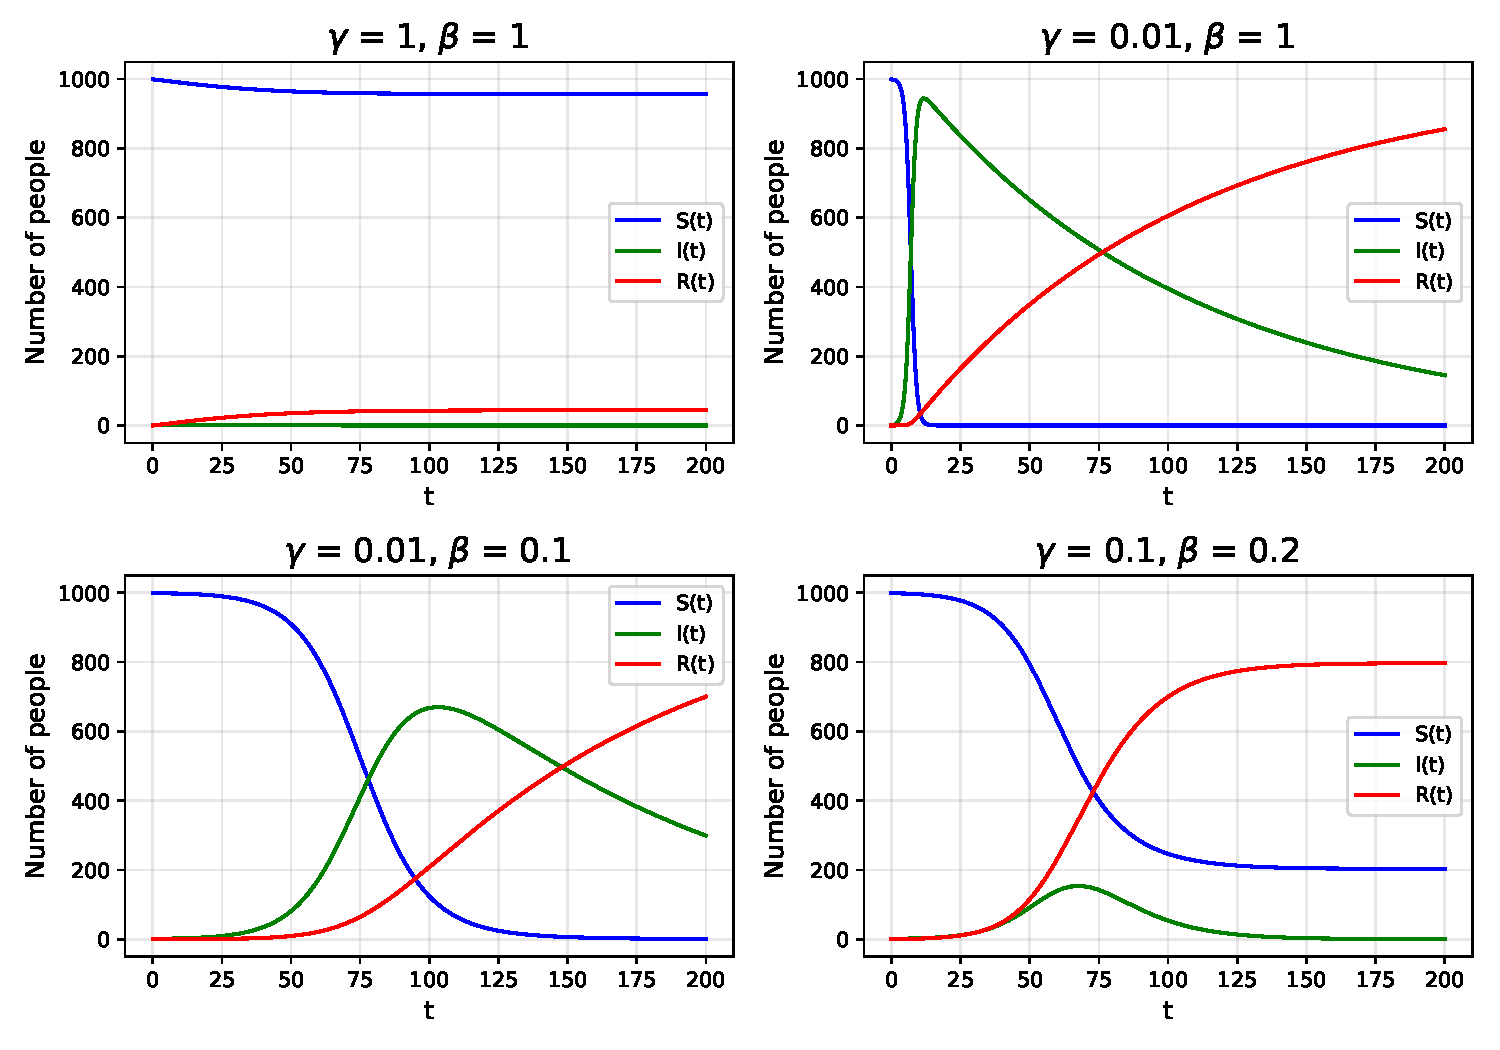
\includegraphics[width=0.8\textwidth]{SIR.pdf}
    \caption{Evolution of the three groups of the population using the SIR model with different $\beta$ and $\gamma$ values.}
    \label{SIR}
\end{figure}

\end{document}
